\documentclass{article} % For LaTeX2e
\usepackage{./iclr2024/iclr2024_conference,times}

% Optional math commands from https://github.com/goodfeli/dlbook_notation.
%%%%% NEW MATH DEFINITIONS %%%%%

\usepackage{amsmath,amsfonts,bm}

% Mark sections of captions for referring to divisions of figures
\newcommand{\figleft}{{\em (Left)}}
\newcommand{\figcenter}{{\em (Center)}}
\newcommand{\figright}{{\em (Right)}}
\newcommand{\figtop}{{\em (Top)}}
\newcommand{\figbottom}{{\em (Bottom)}}
\newcommand{\captiona}{{\em (a)}}
\newcommand{\captionb}{{\em (b)}}
\newcommand{\captionc}{{\em (c)}}
\newcommand{\captiond}{{\em (d)}}

% Highlight a newly defined term
\newcommand{\newterm}[1]{{\bf #1}}


% Figure reference, lower-case.
\def\figref#1{figure~\ref{#1}}
% Figure reference, capital. For start of sentence
\def\Figref#1{Figure~\ref{#1}}
\def\twofigref#1#2{figures \ref{#1} and \ref{#2}}
\def\quadfigref#1#2#3#4{figures \ref{#1}, \ref{#2}, \ref{#3} and \ref{#4}}
% Section reference, lower-case.
\def\secref#1{section~\ref{#1}}
% Section reference, capital.
\def\Secref#1{Section~\ref{#1}}
% Reference to two sections.
\def\twosecrefs#1#2{sections \ref{#1} and \ref{#2}}
% Reference to three sections.
\def\secrefs#1#2#3{sections \ref{#1}, \ref{#2} and \ref{#3}}
% Reference to an equation, lower-case.
\def\eqref#1{equation~\ref{#1}}
% Reference to an equation, upper case
\def\Eqref#1{Equation~\ref{#1}}
% A raw reference to an equation---avoid using if possible
\def\plaineqref#1{\ref{#1}}
% Reference to a chapter, lower-case.
\def\chapref#1{chapter~\ref{#1}}
% Reference to an equation, upper case.
\def\Chapref#1{Chapter~\ref{#1}}
% Reference to a range of chapters
\def\rangechapref#1#2{chapters\ref{#1}--\ref{#2}}
% Reference to an algorithm, lower-case.
\def\algref#1{algorithm~\ref{#1}}
% Reference to an algorithm, upper case.
\def\Algref#1{Algorithm~\ref{#1}}
\def\twoalgref#1#2{algorithms \ref{#1} and \ref{#2}}
\def\Twoalgref#1#2{Algorithms \ref{#1} and \ref{#2}}
% Reference to a part, lower case
\def\partref#1{part~\ref{#1}}
% Reference to a part, upper case
\def\Partref#1{Part~\ref{#1}}
\def\twopartref#1#2{parts \ref{#1} and \ref{#2}}

\def\ceil#1{\lceil #1 \rceil}
\def\floor#1{\lfloor #1 \rfloor}
\def\1{\bm{1}}
\newcommand{\train}{\mathcal{D}}
\newcommand{\valid}{\mathcal{D_{\mathrm{valid}}}}
\newcommand{\test}{\mathcal{D_{\mathrm{test}}}}

\def\eps{{\epsilon}}


% Random variables
\def\reta{{\textnormal{$\eta$}}}
\def\ra{{\textnormal{a}}}
\def\rb{{\textnormal{b}}}
\def\rc{{\textnormal{c}}}
\def\rd{{\textnormal{d}}}
\def\re{{\textnormal{e}}}
\def\rf{{\textnormal{f}}}
\def\rg{{\textnormal{g}}}
\def\rh{{\textnormal{h}}}
\def\ri{{\textnormal{i}}}
\def\rj{{\textnormal{j}}}
\def\rk{{\textnormal{k}}}
\def\rl{{\textnormal{l}}}
% rm is already a command, just don't name any random variables m
\def\rn{{\textnormal{n}}}
\def\ro{{\textnormal{o}}}
\def\rp{{\textnormal{p}}}
\def\rq{{\textnormal{q}}}
\def\rr{{\textnormal{r}}}
\def\rs{{\textnormal{s}}}
\def\rt{{\textnormal{t}}}
\def\ru{{\textnormal{u}}}
\def\rv{{\textnormal{v}}}
\def\rw{{\textnormal{w}}}
\def\rx{{\textnormal{x}}}
\def\ry{{\textnormal{y}}}
\def\rz{{\textnormal{z}}}

% Random vectors
\def\rvepsilon{{\mathbf{\epsilon}}}
\def\rvtheta{{\mathbf{\theta}}}
\def\rva{{\mathbf{a}}}
\def\rvb{{\mathbf{b}}}
\def\rvc{{\mathbf{c}}}
\def\rvd{{\mathbf{d}}}
\def\rve{{\mathbf{e}}}
\def\rvf{{\mathbf{f}}}
\def\rvg{{\mathbf{g}}}
\def\rvh{{\mathbf{h}}}
\def\rvu{{\mathbf{i}}}
\def\rvj{{\mathbf{j}}}
\def\rvk{{\mathbf{k}}}
\def\rvl{{\mathbf{l}}}
\def\rvm{{\mathbf{m}}}
\def\rvn{{\mathbf{n}}}
\def\rvo{{\mathbf{o}}}
\def\rvp{{\mathbf{p}}}
\def\rvq{{\mathbf{q}}}
\def\rvr{{\mathbf{r}}}
\def\rvs{{\mathbf{s}}}
\def\rvt{{\mathbf{t}}}
\def\rvu{{\mathbf{u}}}
\def\rvv{{\mathbf{v}}}
\def\rvw{{\mathbf{w}}}
\def\rvx{{\mathbf{x}}}
\def\rvy{{\mathbf{y}}}
\def\rvz{{\mathbf{z}}}

% Elements of random vectors
\def\erva{{\textnormal{a}}}
\def\ervb{{\textnormal{b}}}
\def\ervc{{\textnormal{c}}}
\def\ervd{{\textnormal{d}}}
\def\erve{{\textnormal{e}}}
\def\ervf{{\textnormal{f}}}
\def\ervg{{\textnormal{g}}}
\def\ervh{{\textnormal{h}}}
\def\ervi{{\textnormal{i}}}
\def\ervj{{\textnormal{j}}}
\def\ervk{{\textnormal{k}}}
\def\ervl{{\textnormal{l}}}
\def\ervm{{\textnormal{m}}}
\def\ervn{{\textnormal{n}}}
\def\ervo{{\textnormal{o}}}
\def\ervp{{\textnormal{p}}}
\def\ervq{{\textnormal{q}}}
\def\ervr{{\textnormal{r}}}
\def\ervs{{\textnormal{s}}}
\def\ervt{{\textnormal{t}}}
\def\ervu{{\textnormal{u}}}
\def\ervv{{\textnormal{v}}}
\def\ervw{{\textnormal{w}}}
\def\ervx{{\textnormal{x}}}
\def\ervy{{\textnormal{y}}}
\def\ervz{{\textnormal{z}}}

% Random matrices
\def\rmA{{\mathbf{A}}}
\def\rmB{{\mathbf{B}}}
\def\rmC{{\mathbf{C}}}
\def\rmD{{\mathbf{D}}}
\def\rmE{{\mathbf{E}}}
\def\rmF{{\mathbf{F}}}
\def\rmG{{\mathbf{G}}}
\def\rmH{{\mathbf{H}}}
\def\rmI{{\mathbf{I}}}
\def\rmJ{{\mathbf{J}}}
\def\rmK{{\mathbf{K}}}
\def\rmL{{\mathbf{L}}}
\def\rmM{{\mathbf{M}}}
\def\rmN{{\mathbf{N}}}
\def\rmO{{\mathbf{O}}}
\def\rmP{{\mathbf{P}}}
\def\rmQ{{\mathbf{Q}}}
\def\rmR{{\mathbf{R}}}
\def\rmS{{\mathbf{S}}}
\def\rmT{{\mathbf{T}}}
\def\rmU{{\mathbf{U}}}
\def\rmV{{\mathbf{V}}}
\def\rmW{{\mathbf{W}}}
\def\rmX{{\mathbf{X}}}
\def\rmY{{\mathbf{Y}}}
\def\rmZ{{\mathbf{Z}}}

% Elements of random matrices
\def\ermA{{\textnormal{A}}}
\def\ermB{{\textnormal{B}}}
\def\ermC{{\textnormal{C}}}
\def\ermD{{\textnormal{D}}}
\def\ermE{{\textnormal{E}}}
\def\ermF{{\textnormal{F}}}
\def\ermG{{\textnormal{G}}}
\def\ermH{{\textnormal{H}}}
\def\ermI{{\textnormal{I}}}
\def\ermJ{{\textnormal{J}}}
\def\ermK{{\textnormal{K}}}
\def\ermL{{\textnormal{L}}}
\def\ermM{{\textnormal{M}}}
\def\ermN{{\textnormal{N}}}
\def\ermO{{\textnormal{O}}}
\def\ermP{{\textnormal{P}}}
\def\ermQ{{\textnormal{Q}}}
\def\ermR{{\textnormal{R}}}
\def\ermS{{\textnormal{S}}}
\def\ermT{{\textnormal{T}}}
\def\ermU{{\textnormal{U}}}
\def\ermV{{\textnormal{V}}}
\def\ermW{{\textnormal{W}}}
\def\ermX{{\textnormal{X}}}
\def\ermY{{\textnormal{Y}}}
\def\ermZ{{\textnormal{Z}}}

% Vectors
\def\vzero{{\bm{0}}}
\def\vone{{\bm{1}}}
\def\vmu{{\bm{\mu}}}
\def\vtheta{{\bm{\theta}}}
\def\va{{\bm{a}}}
\def\vb{{\bm{b}}}
\def\vc{{\bm{c}}}
\def\vd{{\bm{d}}}
\def\ve{{\bm{e}}}
\def\vf{{\bm{f}}}
\def\vg{{\bm{g}}}
\def\vh{{\bm{h}}}
\def\vi{{\bm{i}}}
\def\vj{{\bm{j}}}
\def\vk{{\bm{k}}}
\def\vl{{\bm{l}}}
\def\vm{{\bm{m}}}
\def\vn{{\bm{n}}}
\def\vo{{\bm{o}}}
\def\vp{{\bm{p}}}
\def\vq{{\bm{q}}}
\def\vr{{\bm{r}}}
\def\vs{{\bm{s}}}
\def\vt{{\bm{t}}}
\def\vu{{\bm{u}}}
\def\vv{{\bm{v}}}
\def\vw{{\bm{w}}}
\def\vx{{\bm{x}}}
\def\vy{{\bm{y}}}
\def\vz{{\bm{z}}}

% Elements of vectors
\def\evalpha{{\alpha}}
\def\evbeta{{\beta}}
\def\evepsilon{{\epsilon}}
\def\evlambda{{\lambda}}
\def\evomega{{\omega}}
\def\evmu{{\mu}}
\def\evpsi{{\psi}}
\def\evsigma{{\sigma}}
\def\evtheta{{\theta}}
\def\eva{{a}}
\def\evb{{b}}
\def\evc{{c}}
\def\evd{{d}}
\def\eve{{e}}
\def\evf{{f}}
\def\evg{{g}}
\def\evh{{h}}
\def\evi{{i}}
\def\evj{{j}}
\def\evk{{k}}
\def\evl{{l}}
\def\evm{{m}}
\def\evn{{n}}
\def\evo{{o}}
\def\evp{{p}}
\def\evq{{q}}
\def\evr{{r}}
\def\evs{{s}}
\def\evt{{t}}
\def\evu{{u}}
\def\evv{{v}}
\def\evw{{w}}
\def\evx{{x}}
\def\evy{{y}}
\def\evz{{z}}

% Matrix
\def\mA{{\bm{A}}}
\def\mB{{\bm{B}}}
\def\mC{{\bm{C}}}
\def\mD{{\bm{D}}}
\def\mE{{\bm{E}}}
\def\mF{{\bm{F}}}
\def\mG{{\bm{G}}}
\def\mH{{\bm{H}}}
\def\mI{{\bm{I}}}
\def\mJ{{\bm{J}}}
\def\mK{{\bm{K}}}
\def\mL{{\bm{L}}}
\def\mM{{\bm{M}}}
\def\mN{{\bm{N}}}
\def\mO{{\bm{O}}}
\def\mP{{\bm{P}}}
\def\mQ{{\bm{Q}}}
\def\mR{{\bm{R}}}
\def\mS{{\bm{S}}}
\def\mT{{\bm{T}}}
\def\mU{{\bm{U}}}
\def\mV{{\bm{V}}}
\def\mW{{\bm{W}}}
\def\mX{{\bm{X}}}
\def\mY{{\bm{Y}}}
\def\mZ{{\bm{Z}}}
\def\mBeta{{\bm{\beta}}}
\def\mPhi{{\bm{\Phi}}}
\def\mLambda{{\bm{\Lambda}}}
\def\mSigma{{\bm{\Sigma}}}

% Tensor
\DeclareMathAlphabet{\mathsfit}{\encodingdefault}{\sfdefault}{m}{sl}
\SetMathAlphabet{\mathsfit}{bold}{\encodingdefault}{\sfdefault}{bx}{n}
\newcommand{\tens}[1]{\bm{\mathsfit{#1}}}
\def\tA{{\tens{A}}}
\def\tB{{\tens{B}}}
\def\tC{{\tens{C}}}
\def\tD{{\tens{D}}}
\def\tE{{\tens{E}}}
\def\tF{{\tens{F}}}
\def\tG{{\tens{G}}}
\def\tH{{\tens{H}}}
\def\tI{{\tens{I}}}
\def\tJ{{\tens{J}}}
\def\tK{{\tens{K}}}
\def\tL{{\tens{L}}}
\def\tM{{\tens{M}}}
\def\tN{{\tens{N}}}
\def\tO{{\tens{O}}}
\def\tP{{\tens{P}}}
\def\tQ{{\tens{Q}}}
\def\tR{{\tens{R}}}
\def\tS{{\tens{S}}}
\def\tT{{\tens{T}}}
\def\tU{{\tens{U}}}
\def\tV{{\tens{V}}}
\def\tW{{\tens{W}}}
\def\tX{{\tens{X}}}
\def\tY{{\tens{Y}}}
\def\tZ{{\tens{Z}}}


% Graph
\def\gA{{\mathcal{A}}}
\def\gB{{\mathcal{B}}}
\def\gC{{\mathcal{C}}}
\def\gD{{\mathcal{D}}}
\def\gE{{\mathcal{E}}}
\def\gF{{\mathcal{F}}}
\def\gG{{\mathcal{G}}}
\def\gH{{\mathcal{H}}}
\def\gI{{\mathcal{I}}}
\def\gJ{{\mathcal{J}}}
\def\gK{{\mathcal{K}}}
\def\gL{{\mathcal{L}}}
\def\gM{{\mathcal{M}}}
\def\gN{{\mathcal{N}}}
\def\gO{{\mathcal{O}}}
\def\gP{{\mathcal{P}}}
\def\gQ{{\mathcal{Q}}}
\def\gR{{\mathcal{R}}}
\def\gS{{\mathcal{S}}}
\def\gT{{\mathcal{T}}}
\def\gU{{\mathcal{U}}}
\def\gV{{\mathcal{V}}}
\def\gW{{\mathcal{W}}}
\def\gX{{\mathcal{X}}}
\def\gY{{\mathcal{Y}}}
\def\gZ{{\mathcal{Z}}}

% Sets
\def\sA{{\mathbb{A}}}
\def\sB{{\mathbb{B}}}
\def\sC{{\mathbb{C}}}
\def\sD{{\mathbb{D}}}
% Don't use a set called E, because this would be the same as our symbol
% for expectation.
\def\sF{{\mathbb{F}}}
\def\sG{{\mathbb{G}}}
\def\sH{{\mathbb{H}}}
\def\sI{{\mathbb{I}}}
\def\sJ{{\mathbb{J}}}
\def\sK{{\mathbb{K}}}
\def\sL{{\mathbb{L}}}
\def\sM{{\mathbb{M}}}
\def\sN{{\mathbb{N}}}
\def\sO{{\mathbb{O}}}
\def\sP{{\mathbb{P}}}
\def\sQ{{\mathbb{Q}}}
\def\sR{{\mathbb{R}}}
\def\sS{{\mathbb{S}}}
\def\sT{{\mathbb{T}}}
\def\sU{{\mathbb{U}}}
\def\sV{{\mathbb{V}}}
\def\sW{{\mathbb{W}}}
\def\sX{{\mathbb{X}}}
\def\sY{{\mathbb{Y}}}
\def\sZ{{\mathbb{Z}}}

% Entries of a matrix
\def\emLambda{{\Lambda}}
\def\emA{{A}}
\def\emB{{B}}
\def\emC{{C}}
\def\emD{{D}}
\def\emE{{E}}
\def\emF{{F}}
\def\emG{{G}}
\def\emH{{H}}
\def\emI{{I}}
\def\emJ{{J}}
\def\emK{{K}}
\def\emL{{L}}
\def\emM{{M}}
\def\emN{{N}}
\def\emO{{O}}
\def\emP{{P}}
\def\emQ{{Q}}
\def\emR{{R}}
\def\emS{{S}}
\def\emT{{T}}
\def\emU{{U}}
\def\emV{{V}}
\def\emW{{W}}
\def\emX{{X}}
\def\emY{{Y}}
\def\emZ{{Z}}
\def\emSigma{{\Sigma}}

% entries of a tensor
% Same font as tensor, without \bm wrapper
\newcommand{\etens}[1]{\mathsfit{#1}}
\def\etLambda{{\etens{\Lambda}}}
\def\etA{{\etens{A}}}
\def\etB{{\etens{B}}}
\def\etC{{\etens{C}}}
\def\etD{{\etens{D}}}
\def\etE{{\etens{E}}}
\def\etF{{\etens{F}}}
\def\etG{{\etens{G}}}
\def\etH{{\etens{H}}}
\def\etI{{\etens{I}}}
\def\etJ{{\etens{J}}}
\def\etK{{\etens{K}}}
\def\etL{{\etens{L}}}
\def\etM{{\etens{M}}}
\def\etN{{\etens{N}}}
\def\etO{{\etens{O}}}
\def\etP{{\etens{P}}}
\def\etQ{{\etens{Q}}}
\def\etR{{\etens{R}}}
\def\etS{{\etens{S}}}
\def\etT{{\etens{T}}}
\def\etU{{\etens{U}}}
\def\etV{{\etens{V}}}
\def\etW{{\etens{W}}}
\def\etX{{\etens{X}}}
\def\etY{{\etens{Y}}}
\def\etZ{{\etens{Z}}}

% The true underlying data generating distribution
\newcommand{\pdata}{p_{\rm{data}}}
% The empirical distribution defined by the training set
\newcommand{\ptrain}{\hat{p}_{\rm{data}}}
\newcommand{\Ptrain}{\hat{P}_{\rm{data}}}
% The model distribution
\newcommand{\pmodel}{p_{\rm{model}}}
\newcommand{\Pmodel}{P_{\rm{model}}}
\newcommand{\ptildemodel}{\tilde{p}_{\rm{model}}}
% Stochastic autoencoder distributions
\newcommand{\pencode}{p_{\rm{encoder}}}
\newcommand{\pdecode}{p_{\rm{decoder}}}
\newcommand{\precons}{p_{\rm{reconstruct}}}

\newcommand{\laplace}{\mathrm{Laplace}} % Laplace distribution

\newcommand{\E}{\mathbb{E}}
\newcommand{\Ls}{\mathcal{L}}
\newcommand{\R}{\mathbb{R}}
\newcommand{\emp}{\tilde{p}}
\newcommand{\lr}{\alpha}
\newcommand{\reg}{\lambda}
\newcommand{\rect}{\mathrm{rectifier}}
\newcommand{\softmax}{\mathrm{softmax}}
\newcommand{\sigmoid}{\sigma}
\newcommand{\softplus}{\zeta}
\newcommand{\KL}{D_{\mathrm{KL}}}
\newcommand{\Var}{\mathrm{Var}}
\newcommand{\standarderror}{\mathrm{SE}}
\newcommand{\Cov}{\mathrm{Cov}}
% Wolfram Mathworld says $L^2$ is for function spaces and $\ell^2$ is for vectors
% But then they seem to use $L^2$ for vectors throughout the site, and so does
% wikipedia.
\newcommand{\normlzero}{L^0}
\newcommand{\normlone}{L^1}
\newcommand{\normltwo}{L^2}
\newcommand{\normlp}{L^p}
\newcommand{\normmax}{L^\infty}

\newcommand{\parents}{Pa} % See usage in notation.tex. Chosen to match Daphne's book.

\DeclareMathOperator*{\argmax}{arg\,max}
\DeclareMathOperator*{\argmin}{arg\,min}

\DeclareMathOperator{\sign}{sign}
\DeclareMathOperator{\Tr}{Tr}
\let\ab\allowbreak


\usepackage{hyperref}
\usepackage{url}
\usepackage{charter}
\usepackage{eulervm}
\usepackage{graphicx} 

\usepackage{amssymb,amsmath}
\usepackage{wrapfig}
\usepackage{booktabs}

\renewcommand{\arraystretch}{1.2}

\usepackage[T1]{fontenc}% NOT OT1
\usepackage[scaled]{beramono}
%\usepackage{inconsolata}
\usepackage{listings}
\lstset{basicstyle=\ttfamily\small}

\makeatletter
\renewcommand*{\verbatim@font}{}
\makeatother

\definecolor{my-green}{HTML}{677d00}
\definecolor{my-light-green}{HTML}{acd373}
\definecolor{my-lighter-green}{HTML}{e6ecce}
\definecolor{my-red}{HTML}{b13e26}
\definecolor{my-light-red}{HTML}{d38473}
\definecolor{my-blue}{HTML}{306693}
\definecolor{my-light-blue}{HTML}{73a7d3}
\definecolor{my-gray}{HTML}{999999}
\definecolor{my-orange}{HTML}{E69500}
\definecolor{my-light-orange}{HTML}{FFC353}
%
%\usepackage[colorlinks=true,citecolor=my-red,urlcolor=my-green,linkcolor=my-red]{hyperref}

\newcommand{\lgcl}[1]{{\color{my-light-green} #1}}
\newcommand{\gcl}[1]{{\color{my-green} #1}}
\newcommand{\lrcl}[1]{{\color{my-light-red} #1}}
\newcommand{\rcl}[1]{{\color{my-red} #1}}
\newcommand{\lbcl}[1]{{\color{my-light-blue} #1}}
\newcommand{\bcl}[1]{{\color{my-blue} #1}}
\newcommand{\kcl}[1]{{\color{my-gray} #1}}
\newcommand{\locl}[1]{{\color{my-light-orange} #1}}
\newcommand{\ocl}[1]{{\color{my-orange} #1}}

\newcommand{\h}[0]{\hspace{0.12em}}


\title{Universal pre-training}

% Authors must not appear in the submitted version. They should be hidden
% as long as the \iclrfinalcopy macro remains commented out below.
% Non-anonymous submissions will be rejected without review.

\author{Peter Bloem \\
Learning \& Reasoning Group\\
Vrije Universiteit \\
Amsterdam, Netherlands \\
\texttt{up@peterbloem.nl} \\
}

% The \author macro works with any number of authors. There are two commands
% used to separate the names and addresses of multiple authors: \And and \AND.
%
% Using \And between authors leaves it to \LaTeX{} to determine where to break
% the lines. Using \AND forces a linebreak at that point. So, if \LaTeX{}
% puts 3 of 4 authors names on the first line, and the last on the second
% line, try using \AND instead of \And before the third author name.

\newcommand{\fix}{\marginpar{FIX}}
\newcommand{\new}{\marginpar{NEW}}

\newcommand{\B}{\mathbb B}
\newcommand{\p}{\text{.}}
    


\iclrfinalcopy % Uncomment for camera-ready version, but NOT for submission.
\begin{document}


\maketitle

\begin{abstract}
We investigate the use of randomly generated data for the sake of pre-training a model, \emph{before} seeing any domain-specific data. We justify this approach theoretically from the perspective of Kolmogorov complexity. We show empirically, in the domain of token sequences, that randomly generated data can be used to pre-train a model a-priori---before the data is seen---and that this leads to a certain amount of absolute, zero-shot in-context learning. That is, for simple tasks, the resulting model is able to learn in-context without seeing any training data. We call this approach \emph{universal pre-training} and we invistigate several potential benefits. First, it leads to better-than-chance zero-shot performance. That is, the model shows some in-context test-set performance before seeing \emph{any} training data. Second, when the model is fine-tuned on training data after pretraining, it converges faster and to better performance, even when the pretraining is accounted for in the computational budget. And third, The resulting model shows better generalization both in-domain and out-of-domain. While these experiments are only small-scale, we perform a scaling experiment that shows a promising trend towards larger models.
\end{abstract}

\section{Introduction}



Even in the domain of natural language, where vast amounts of data are available, machine learning is fast approaching the point where the amount of data on which we would like to train a model is larger than the total amount data available \cite{}. In many other domains, this point has long been passed. At the same time, as artificial intelligence becomes more and more integrated in production systems, producers of, for instance, literature and art, are less eager for their work to end up in training datasets. In short the question of whether we can do more with less data is increasingly urgent.
%
\begin{wrapfigure}{r}{0.55\textwidth}
		\vspace{0em}
        \begin{minipage}{0.55\textwidth}{}
        \begin{tabular}{l l}
			(a) & \lstinline|Z'WY,!X#R_M!IK@JQ!?.>Z\_0&2L%V2G1D4'!| \\
			\hline
			(b) & \lstinline|;5;;'6BUB5CBBBB5Z55BX'X5ZUZZ5P%X555Z5| \\ 
                & \lstinline|E$QFGQ.!XQN*Q,.!.,G**GFFFFF^^FPQ^!YQF| \\
				& \lstinline|\^R5D#**JI,DTTTT,TTTS\TITIDSDT*TTTT\\| \\
				& \lstinline|AFFFFFFFFFFFF\FFFFFFF!\FFFFFF;FFFFFFF| \\
		\end{tabular}
        \end{minipage}

        \caption{An example of the main idea behind our approach (a) A string of uniformly sampled ASCII characters. (b) The result of passing this string through four randomly initialized models. Note that in (b), we can to some extend precict whcih characters we will see from which characters came before. This gives (b) some value in pre-training.}
        \label{fig:example}
        \vspace{-0.5em}
\end{wrapfigure}
% 


One approach is to generate \emph{synthetic data}. This may seem at first to be a false economy: how can we learn something from a data generator that we built ourselves? In information theoretic terms, the data processing inequality (DPI) \cite{} tells us that we cannot increase the information content of a signal by applying computation to it. This seems to preclude the possibility of enriching our models with data from any other source than the real world.

However, the key to valuable data is not information content, it's \emph{structure}. The most information-rich signal, a fully random one, is among the least valuable data to learn from. A valuable source of data provides a mix of randomness and structure.

Consider the following analogy (from \cite{}). A monkey behind a typewriter, bashing keys at random, will famously produce the complete works of Shakespeare in a large, but finite amount of time. A monkey behind a \emph{computer} will also produce the collected works of Shakespeare, and \emph{it will do so more quickly}. This is because there is structure in natural language that may be exploited by a computer program. The second monkey only needs to be lucky enough to type out a computer program that produces the collected works of Shakespeare, whereas the first monkey needs to be lucky enough to get every single character correct.

The key takeaway is that by taking a source of randomness---whether a monkey or a random number generator---and passing its output through a computer, we can \emph{enrich} data (from the perspective of machine learning). This may well reduce the amount if information in the data (in the Shannon/Kolmogorov sense of the word), but it adds structure. Structure that a machine learning model can learn, and that may transfer to real-world tasks.

With this principle in mind, we ask the following question. Can we pre-train a model before seeing the data? Can we generate rich random data, before knowing what our task is, such that pre-training on this random data benefits learning, regardless of the task? We show that this is indeed possible, and we call the resulting approach \emph{universal pre-training}. We provide some theoretical foundation for this principle, from the field of Kolmogorov complexity.

Figure~\ref{fig:example} shows a simple example of our approach: a string of ASCII characters, each chosen uniformly at random, and the result of passing that string through a randomly initialized transformer model. The first string is fully random, and nothing useful may be learned from it. The second string contains structure: certain characters and structures re-occur in a predictable way. We can make sensible predictions about one part of the string by studying another part of the string. 

\begin{figure}[t!]

  \centerline{\hspace{-1.2em}
    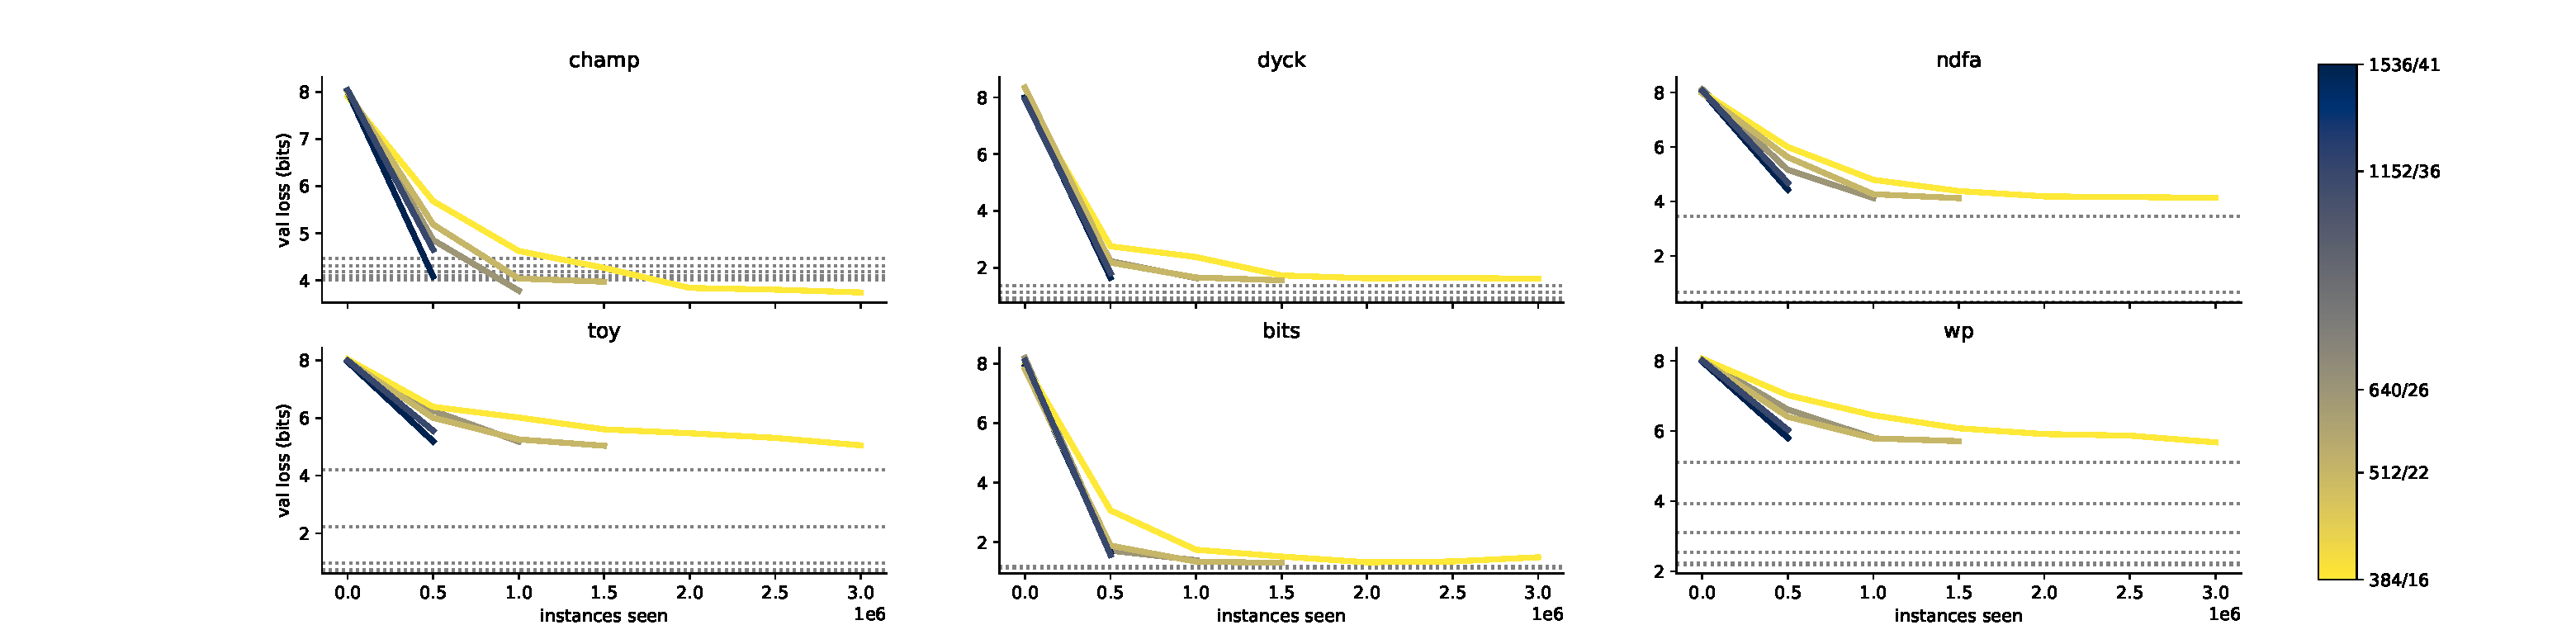
\includegraphics[width=1.3\textwidth]{./figures/scaling.pdf}
  }
  \caption{The results of the main scaling experiment (Section~\ref{section:scaling}). We train a transformer model on randomly generated data with computational structure, and test its prediction performance, zero-shot on six simple datasets. Horizontal lines indicate the performance of an $n$th-order Markov model (with orders $0$ -- $4$). The results show that the zero-shot behavior (a) is better than chance across the board (b) in some cases beats the performance of a domain-specific Markov model (c) \emph{improves with scale}.}
  \label{figure:scaling}
\end{figure}

Some of these basic patterns may transfer to other domains. For instance, the relative frequency of a character at the start of the string, is more likely than not be a reasonable prediction of its probability at the end of the string, and this pattern will hold across a wide variety of tasks.

 Other patterns, such as the specific characters that are frequent, are entirely specific to the current sample, and will disappear if we sample a second string in the same way.

Ultimately, if universal pre-training works well, patterns that are likely to be \emph{universal}---that is, shared by many datasets generated from computational sources---will be learned by the model, whereas patterns that are specific only to very specific sources, will quickly be averaged out. 

Our contributions are threefold:
\begin{itemize}
\item We provide a theoretical framework to show that, under certain assumptions, universal pre-training may be used to invest compute to improve model performance before seeing the data. That is, to trade off compute for data (if at a high cost). 
\item We introduce a simple algorithm for generating structured data by passing random data through a randomly initialized transformer model. We use a buffering approach to allow for batched computation, while still generating approximately iid samples.
\item We show that pre-training a model on data generated in this way, leads to better than chance zero-shot in-context learning performance on various toy and real-world tasks, and that this performance improves with scale. 
\end{itemize}

The final point is particularly relevant. While we find that a substantial amount of computation is currently required to reach the zero-shot performance of even a simple Markov model, this investment could, in principle be amortized over many downstream tasks if the benefit is truly universal. Taking together with the scale of modern machine learning training, there may already be a benefit. 

In the conclusion, we suggest a series of key research directions that should be pursued to establish whether universal pre-training may become a viable approach at scale, in the future. We also pause to consider what the impact may be, if this data/compute tradeoff is chased blindly in, based on optimistic predictions.

\section{Preliminaries}

We will briefly review the required preliminaries. See \cite{} for a more detailed treatment. These are mostly required to understand the theoretical framework we use to show that universal pre-training is feasible. To understand the experimental part of the paper, the intuitive explanation in the introduction should suffice.

Let $\B$ be the set of finite binary strings $\{0, 1, 00, 01, 10, 11, 000, \ldots\}$. We will use Turing machines \cite{} to model computable probability distributions on $\B$. To this end we, fix Turing machines with a single input tape and a separate output tape. The read-head on the input tape is only allowed to move from left to right: the effect of this constraint is that after reading a bit from the input tape, the machine either halts, reads the next bit, or computes infitenly without doing either. This means that the set of inputs on which a machine halts forms a prefix-free set: no halting input is the prefix of another halting input.  This is called a prefix-free Turing machine \cite{}.

If a machine $T$ halts, we take the input bits it has read as its input $x$, and the value on its output tape when it halts as its output $y$, writing $T(x) = y$. We write $T(x)=\infty$ for an input on which the machine does not halt (that is, it processes indefinitely without advancing the read head).

We can now use such machines to simulate probability distributions, by feeding them random bits. We start the machine, and whenever it reads from the input tape, we sample a random bit and provide it. If the machine halts, we take the output as our sample.\footnotemark

\footnotetext{Since the machine may not halt, this is a deficient distribution on $\B$. However, we will mostly deal with subsets of the Turing machines that always halt. If we place no restrictions on the Turing machines used, we have defined the class of \emph{lower semicomputable semimeasures} \cite{}. We will refer to these as the computable distributions for the sake of simplicity.}

We assume that we are given some enumeration $T_i$ of all Turing machines, with $i\in 0, 1, 2, \ldots$. We refer to the probability of sampling $y$ from $T_i$ as $p_i(y)$. Since each input $x$ is sampled with exactly probability $2^{|x|}$, where $|\cdot|$ denotes string length, we can write $p_i$ as

$$
p_i(y) = \sum_{x : T_i(x) = y} 2^{|x|} \p  
$$

Next, assume a pairing function $(i, x)$ that encodes $i$ and $x$ into a single string in $\B$, then we can define a universal Turing machine $U((i, x)) = T_i(x)$, which unpacks the string $(i, x)$ function and then simulates the running of the $i$-th Turing machine on input $x$. If the pairing function uses prefix-free codewords, which is easy to achieve, then $U$ is itself a prefix-free Turing machine, which means that  occurs somewhere in the enumeration $T_i$. \footnotemark

\footnotetext{A simple way to achieve a prefix-free pairing function is to define a prefix-free encoding of $\B$, written as $\bar x$. We can then use the pairing function $(i, x) = \bar \imath\bar x$, since concatenating two prefix-free codewords results in another prefix-free code.}

With this, we can sample from $U$, feeding it random bits until it halts. This effectively samples a Turing machine $i$ according to some prior probability $p(i)$, and then samples an output $y$ according to  $p_i(y)$. We call this the \emph{universal distribution} $m(y)$. The universal distribution is a Bayesian mixture over the class of computable distributions.

\section{Related work}

\subsection{Synthetic data}

Training on synthetic data goes back to the simple principles of data augmentation \cite{}. In recent years, much research has been devoted to the use of simulators generating synthetic data to encode very specific domain assumptions. For instance, in training self-driving cars, robotics control, tabular data, ... \cite{}.

Our work follows this trend, but with the change that we aim to make the assumptions on the domain \emph{minimal}. In its most general form, universal pre-training only assumes that the source of the downstream dataset is \emph{computational} in nature. This allows one form of pre-training to be used for a wide variety of downstream tasks.

\subsection{The No-Free Lunch Theorem}

The idea of pre-training a model irrespective of its task seems to fly in the face of the no-free-lunch (NFL) theorem \cite{}, which states that, averaged over all tasks, all models perform the same. This suggests that if our pre-training makes any change at all to the model's performance on a subset of tasks, it must reduce its performance on other tasks.

This is indeed true, but it's possible to get out of the NFL theorem with a very broad, almost universal assumption about our data: that the process $p$ that generated it is \emph{computational}. That is, it can be simulated by a probabilistic Turing machine. Under this assumption, the source of our data is \emph{dominated} by the universal distribution $m$, and by any class-universal distribution $m_C$ for which $p \in C$. 

This means that there are computable probability distributions $m_C$ that fit our data as well as its source $p$ does (up to a multiplicative constant). Moreover, this holds for all $p \in C$. Therefore, $m_C$ provides a universal predictor for $C$. This does not violate the NFL theorem, because we do make an assumption about the data, namely that it comes from a source in $C$. However, $C$ can be made \emph{very} broad, for instance the class of all polynomial-time Turing machines, while still allowing practical sampling.

By training on samples from $m_C$, we are essentially approximating it in our pre-trained model.\footnotemark

--Yuki Asano's work.
--Max Welling, amortization

\section{Method}

We will first build on the preliminaries to establish some useful theoretical properties. We then use these to inform a practical first attempt at universal pre-training in the context of sequential transformer models. Since this is intended as a first proof-of-concept, some aspects of the theoretical settings will be dropped for the sake of practicality.

\subsection{In theory}

Let $C$ be a set of computable functions from $\B$ to $\B$. If we define some prior $m_C$ on $C$, we can sample a random model from $C$, feed it random bits $r$, and observe the output $x$. The probability of sampling some specific $x$ from this process is 
\[
p(x) = \sum_{c\in C,r \in R} m_C(c)\;2^{-|r|} \;\;\;\text{with}\;\;\; R = \{r \mid c(r) = x\}\p 
\]

By the logic spelled out in the introduction, this output is more likely to contain interesting structure than the original random bits. We could proceed by pre-training a model on samples from $p$ directly, but we can enhance the depth of our data still more. 

The idea is that if taking a uniform random string and passing it through a computable function can produce `interesting' data, then it's possible that taking such interesting data and passing it through a computable function again, can create even more interesting data. 

That is, if we take the output of the monkey behind the computer, and have it dictate the keypresses of another monkey behind a computer, are we even more likely to produce Shakespeare? If the computers are universal, we cannot boost its power this way: the universal computer cannot be made mode powerful by connecting it to another universal computer. However, if the resources of the computer are limited, we can, chaining together computers increases the overall resources available. For instance, if the computer is only allowed to run for 1 minute, this provides a computer that is allowed to run for 2 minutes. We can make use of this by using both outputs (from the first and second computer) as training data, giving the equivalent of three minutes of computation time in interestingness while we have spent only one.\footnotemark

\footnotetext{This is not without downsides. What we give up is the iid. nature of our generated data. However, in practice, we find that the complicated relation between the two strings is unlikely to affect the training behavior of an algorithm as simple as gradient descent.}

Before we work this into a practical algorithm, we will formalize and prove this intuition as follows. Let $p_u$ be a base distribution on $\B$ which is uniform in the sense that all strings of the same length have equal probability.

Let $m^1_C = m_C$ be the distribution defined by the process of sampling $u$ from $p_u$ and $c$ from $p(C)$ and computing $c(u)$. Then, let $m^{n+1}_C$ be the distribution defined by the process of sampling $u$ from $m^n_C$ and $f$ from $p(C)$ and computing $f(u)$.

\subsection{In practice}

To test these ideas in practice, we make the following simplifications and implementation choices. 

First, instead of training on sequences of bits, we take our token alphabet from the expected downstream task. These are ASCII characters in the first experiment and WordPiece tokens in the second. While this does reduce the universality of our approach somewhat, it suffices for a proof-of-concept (see also the discussion).

For ease of implementation we limit ourselves to sequences of a fixed length. This makes memory use predictable. Our class of source models $C$ is a model class of single-stack transformers with causal self-attention. The architecture is detailed in the appendix. We sample from $C$ simply by initializing its parts using the standard algorithm for the part (also detailed in the appendix), and then scaling all parameters by a fixed constant afterwards. 

For efficiency and ease of implementation, we initialize a single model $f_i$, and sample a batch of $n$ instances from it. This means that the batch is \emph{not} independently sampled from $m_C$. Training directly on such batches would create a bias at each gradient update for the patterns that are specific to $i$. 

To approximate independent sampling, we instead keep a buffer of $k$ samples. Each iteration, we take $n$ instances $x$ from the buffer and replace them by $f_i(x)$. We then sample $n$ random instances again for our target model to train on. We also replace a small proportion $\alpha$ of instances in the buffer with (pseudo-)random noise, to stop the amount of entropy becoming to low.

While this does not fully ensure that the samples are independent, it does ensure that with high probability, each instance in a training batch was generated from a different model $i$.

Moreover, because we are sampling structured noise, and feeding it back into the data, Theorem~\ref{} tells us that we are approximating a sample from a mixture over the infinite sequence of models $m^1_C, m^2_C\ldots$, while only passing one batch of instances through one model from $C$ (the cost of a direct sample from $m^1_C$).\footnotemark
\footnotetext{The probability of a sample coming from $m^n_C$ decays exponentially with $n$, so this claim should be taken with a pinch of salt. However, the ablation in section \ref{} shows that this resampling from the buffer does have a beneficial effect. }

The complete algorithm is detailed in Algorithm~\ref{}.

On these samples, we train a standard autoregressive transformer (architecture and training details in the appendix) by shifting the sequences one character to the left to form the target value, so that the model is trained to predict the next character at each position.

\section{Experiments}

\subsection{Downstream data}

We evaluate on five synthetic sources of data. Each consists of a generator that produces strings of ASCII characters, possibly of variable length.  We sample sequences and concatenate them with a single delimiter character ``\texttt{|}'' until the total exceeds 100\h000 characters. 
 
\begin{description}
\item[\texttt{champ}] Inspired by the Champernowne constant\footnotemark, this source generates successive integers, and outputs their concatenated digits as tokens. We sample a starting integer at random from $[0, 16777216-256]$ and then concatenate it together with the subsequent 255 integers in a string, the characters of which are tokens. The idea behind this dataset is that there is a simple computational structure that allows perfect predictions, but a simple, low-order Markov model will not be able to exploit this structure.
\item[\texttt{dyck}] Generates \emph{Dyck words}: that is, sequences of opening and closing brackets, such that each opening bracket is closed with no closing brackets left over. The result is that a simple predictor can get good performance by always predicting ``('' or ``)'' with equal probability and ``\texttt{|}'' with small probability (as a $0$-order Markov model would do), a perfect predictor would only assign non-zero probability to ``\texttt{|}'' when the preceding string forms a Dyck word. 
\item[\texttt{ndfa}] A string generated from a simple, non-deterministic automaton, shown in Figure~\ref{figure:generators}.
\item[\texttt{ndfa}] A string generated from a simple toy grammar, shown in Figure~\ref{figure:generators}.
\item[\texttt{bits}] Each string consists of two random strings of 5 bits, followed by the result of applying the operators xor, $\wedge$, $\vee$ and $=$ respectively for a sequences of 30 bits. The first 10 of these are fully random, while the last 20 are fully determined by the   first 10. Including the delimited, a perfect predictor, given sufficient context would get a performance of $10/31 \approx 0.32$ bits.
\end{description}

In addition, we include one real-world dataset called \textbf{\texttt{wp}}: the validation set of the Hutter prize Wikipedia data (also known as \texttt{enwik8}). The data is loaded as a sequence of bytes, so that some special characters are represented as two tokens. It is unlikely that a model should learn to predict English characters with any degree of accuracy from a 512-character snippet in a zero-shot setting, so this data serves more to show the complexity gap between the synthetic datasets and real-world data.

We estimate the binary negative log-likelihood of a given model in this data. The characters are mapped to the tokens of the model $m$ by their ASCII code.\footnotemark We sample 1\h000 slices of context length from the data and average the negative binary log-probability that the model assigns to the character in the last place of the sequence. Note that we treat the whole data as a single string, so that the delimiters, \texttt{|},  are included (and may end up anywhere in the sampled slice).

\footnotetext{Note that this mapping is arbitrary, since the model has not been trained on this data.}

\footnotetext{$0.\rcl{1}2\rcl{3}4\rcl{5}6\rcl{7}8\rcl{9}10\rcl{11}12\rcl{13}\ldots$ One important property is that no $n$-gram occurs more frequently than any other in the decimal expansion. That means a Markov model would not be able to predict the next character better than chance. However, there is a simple program that can perfectly predict the next character.}

\subsection{Models}

\subsection{Scaling}

\subsection{Ablation}

\paragraph{Source depth} In our scaling experiments, we scale the source model up at the same rate as the target model. While this could in theory lead to more computationally rich data, this is not guaranteed, and it may be that a model of 40-layers deep will learn that same patterns from a 40 layer source model as it would from a 3-layer source model. 

To investigate, we retrain the model of width 1536 and depth 41 and re-train it with 5 source models of different width. We adjusting all other parameters in the same way as in our scaling experiment. The results are shown in Figure~\ref{figure:ablation-1}.

\paragraph{Other data} As a point of comparison, it's useful to see how a model performs on these tasks when it's trained on different sources of data. It may be, for example, that any training results the observed results and scaling behavior.

First, we train on two further sources of random data: fully random data (which we do not expect to yield a benefit) and data from an $n$-th order Markov model. We train each on a model with width $512$ and depth $22$ for 3M instances. Finally, we train a model in the Wikipedia training data, to see how much of a ``universal'' benefit NLP data provides.\footnotemark

The results are shown in Figure~\ref{figure:ablation-markov}.

\footnotetext{Note that the Wikipedia data contains a great deal of structured text beyond what is normally found in NLP data, for instance in the wiki-markup, in URLs and in various snippets of XML.}

\section{Discussion}

There are three main ingredients in the modern machine learning process that limit how well we do: the fundamental abilities of the algorithm, the available amount of data and the available amount of computational resources. This paper shows that, at least to some extent, it is possible to trade off computational resources for data. We can generate structured random data to pre-train our models, making them require less real-world training data by comparison.

Moreover, the pre-training is in some sense universal. That is, the same pre-training can benefit a large amount of downstream tasks. This allows us to amortize the pre-training over many different tasks, reducing the cost of the tradeoff. 

\subsection{Limitations and Future Work}

\paragraph{approximation of $m_C$} We can show that $m_C$ is a universal model for any $p\in C$. We then proceed by approximating $m_C$ by training a model on samples from it. However, the model we use is not much more complex than $p$.

There is no guarantee that a simple model that is not much more complex than $p$ can simulate $m_C$. Generally, it's likely the case that $m_C$ needs to be of higher complexity than any element in $C$.\footnotemark

\footnotetext{There aren't (to the best of our knowledge) any non-trivial separation proofs. } 

In our work we simply give our model which approximates $m_C$ the same complexity as the models in $C$. It's unlikely that this leads to a convergent approximation, even in optimal conditions. Most likely the approximation simply lacks the required computational complexity. 

For the time being, without any theoretical guarantees we simply assume that an imperfect approximation of $m_C$ is still likely to produce effective pre-training for any task in $C$, and proceed empirically. This leaves several theoretical questions unanswered: (a) what is the computational complexity of $m_C$? (b) Under what conditions is $m_C$ effectively learnable? (c) If there are fundamental limitations in our learned approximation of $m_C$, what are the implications for the effectiveness pre-training?

In short, we use our theoretical framework to show what is possible \emph{in principle}, despite seeming objections from results like the NFL theorem. We then show experimentally, that the expected results can, in at least one domain, be achieved. However, the theoretical framework is insufficient, as yet to say anything about when universal pre-training is guaranteed to work. We leave this to future work.

\paragraph{Universality of assumptions} Calling the specific approach used in our experiments \emph{universal} is an overstatement. We do not sample from a universal distribution (which is not tractable). A class-universal distribution with a sufficiently broad class (like $P$) would still justify the name universal pre-training (since it's very likely that all data sources are in that class), but we fall short of that as well.

First, in the interest of efficient generation, our class $C$ is limited to finite strings, and to the transformer architecture. While the stacking trick allows arbitrary sampling depths (in theory), this does not necessarily mean that we are sampling from the distribution on arbitrarily deep transformers. First, because the probability of sampling at depth $n$ decays exponentially with $n$ in our algorithm and second because the sampling of tokens at the end of each individual pass removes information that an arbitrarily deep transformer may keep in its hidden activations. 

Moreover, we have manipulated the specifics of the source model somewhat to generate data that looks, on inspection, like it contains reasonable structure. This may provide some bias towards the kind of patterns that are likely to appear in our downstream tasks. 

In short, while the framework as we have described it, in its most general terms deserves the moniker \emph{universal}, our practical implementation of it is more of an approximation to this ideal.

\paragraph{Other domains} Our experiments are limited to token sequences. That is, strings of tokens from a finite vocabulary. In principle, the same idea could be applied to computer vision, continuous time series and any other domains. Ideally, those domains would be unified in a single data representation so that one universal model may be applied to all. We leave this to future work.

\paragraph{Other computational sources} For ease of implementation, we use the same type of model for our source of randomness as for our pre-trained model. this is not strictly necessary. For instance, we could easy sample probabilistic string models from different levels of the Chomsky hierarchy. These models can be sampled very efficiently, and may allow more interesting structure to emerge more quickly than it would from our source model. In general, what sources of structured random data will lead to the best (universal) downstream performance is a an open question that may only be resolved through a great deal of experimentation. There may also be a tradeoff between efficiency and universality. 

\section{Social impact}

At the time of publication, large model development is experiencing something of an exponential growth. Some commentators have already suggested that this is a bubble, driven by overoptimistic predictions of future payoffs \cite{}.

The limited availability of high-quality data functions as a limiter on this exponential growth. Training models beyond a certain size is no longer feasible, not because companies are not willing to invest the money and energy, but because the data is either not available, or it is too expensive to acquire the rights.

We have shown that, at least in principle, compute may be traded off against data. We stress that it remains to be seen how this effect plays out at scale, and it may never become economical to do so. However, if it does turn out to be a viable tradeoff, an important limiter on the explosive investment will disappear. 

We need only look at developments like crypto-currency to see how far people  will collectively go to invest in a promised future reward, with amounts of energy at the scale of countries going into a technology that has far from proven its value. In short, there is a risk of an even greater run on energy consumption for training AI models than we are already seeing, at a time when climate change dictates that we should be strictly scrutinizing our energy consumption.

On the other hand, universal pre-training may also provide a middle ground. Since a model trained in this way is guaranteed not to contain any sensitive data, and may be used in a variety of tasks, the training of such models may be centralized, with the result easily published under a free license. While the cost of training will still be substantial, it can then be amortized over all users, rather than just the use regulated by a single company. So long as we can prevent a multitude of companies duplicating the same effort in a race to the biggest proprietary model, the net impact may be a positive, reducing the amount of energy the average user spends on training AI models.

\subsubsection*{Acknowledgments} Experiments for this research were run on the DAS6 \cite{} and Snellius \cite{} super computers.

\bibliography{iclr2024_conference}
\bibliographystyle{iclr2024_conference}

\appendix
\section{Appendix}
You may include other additional sections here.

\end{document}
